
\documentclass[12pt]{article}
\usepackage{graphicx}
\usepackage{booktabs}
\usepackage{setspace}
\doublespacing
\usepackage[np]{numprint}
\npstyleenglish

\begin{document}
	\title{16S RNA Sequencing Data Management using SQLite}
	\author{Xu Junjie, Kevin}
	\date{June 2014}
	\maketitle
	\begin{abstract}
		The 16S Ribosomal RNA Sequencing is used extensively in analzying bacterial
		phylogeny and taxonomy. This project attempts to streamline the 16S sequencing
		pipeline using local file databases to replace multiple flat sequence files used
		in the pipeline, to ease logistical burdens on the researcher and enable 
		greater metadata analysis and accountability of experiments.
	\end{abstract}
	\tableofcontents
	\section{Introduction} % (fold)
	\label{sec:introduction}
	The project utilized computational methods such as 16S Ribosomal Profiling as a proxy for species identity. The 16S small subunit of bacterial ribosomes are highly conserved, which means that the differences within the 16S RNA profiles can be used as an analogue for species identity. Since the 16S gene contains both highly conserved and highly variable regions all interspersed together,
	The highly conserved regions can be amplified using PCR (Polymerase chain reaction), while the variable regions are used to classify the organism. HTS (High Throughput Sequencing) using Illumina sequencers are then used to sequence the PCR products from the prior step.

	The output from HTS forms the start of the computational pipeline. In the preprocessing stage, poor quality reads are filtered and trimmed. Chimeras and non-bacterial 16S reads are then removed. The pipeline then attempts to produce phylogenetic classification through the use of RDP classifiers and sequence similarity (i.e. OTU Analysis). By comparing the filtered output from HTS against the already existing taxonomies of over 2 million species, the genus, family, and order of the sample can be determined.

	The RDP classifier can fail for various reasons: the majority of bacterial species have not been identified or sequenced, the 16S reads are usually too short for accurate classification. In those cases, groups of highly similar sequences are grouped into OTUs (Operational Taxonomic Unit) that can be analyzed for
	quantitative differences in communities between the sequenced samples.

	The project utilizes a computational approach due to the large amount of raw sequencing data that is created from the PCR amplification process. The variability of results is further affected by the OTU Analysis stage, where prior parameters can affect the analysis outcome. Using a computational approach would allow the change of various parameters, in order to quantitate the effects of those parameter changes.

	The majority of the pipeline is executed on the University of Oregon’s ACISS High-Performance Supercomputer Cluster, and utilizes PBS scripts (normal shell scripts with extra variables defined to manage job resources) to execute the different stages of the pipeline.

	The FASTQ output produced by the Illumina sequencer is run through the preprocessing stage of filtering, trimming, and demultiplexing. The PBS script for the preprocessing stage calls on the Demultiplexer, a python script written by Rodger Voelker, which removes the primer attached to the sequences during the amplification process, and attaches barcodes (signifying sample origin) to both ends of the paired-end reads in the FASTQ file. After demultiplexing, the pipeline proceeds to use Trimmomatic v0.32, an open source tool to trim poor quality feeds from the reads. It uses a sliding window trimming, that cuts out sequences when the average quality within a window falls below a certain threshold. Finally, Bowtie 2.1.0 is used to align the reads to existing mitochondrial and phiX sequences and to remove them.
	
	% section introduction (end)
	\section{Data Management} % (fold)
	\label{sec:data_management}
	Data in the pipeline is conceptually divided into three tasks:
	
	\begin{enumerate}
		\item Storing sequence data in a compressed form
		\item Transforming stored data into a format required by tools in the pipeline
		\item Logging metadata
	\end{enumerate}

	\subsection{Database Structure} % (fold)
	\label{sub:database_structure}
	The database is initialized with 4 tables:

	* primer - holds all the primers used in experiment
	* offset - randomized offsets to aid 16S sequencing
	* barcode - experiment identifier
	* log - holds logging data to aid accountability in experiments
	
	The log table supports the logging of metadata and a record of all operations done on the database.
	How to describe metadata logging? What sort of metadata are we planning to capture?

	General logging can be described in accountability terms - e.g. time of operation, tables operated on,
	number of rows operated, who (email? username?) operated. Purpose of this table
	is to automatically record operations so experiments can be reproduced with the
	appropriate settings/parameters easily.

	During the process of importing FASTQ data into the database, another table is produced:

	* reads1,reads2 - holds paired-end FASTQ data
	* reads - holds single-end FASTQ data
	% subsection database_structure (end)

	\subsection{Data Compression} % (fold)
	\label{sub:data_compression}
	Short description of the compression scheme (combining sequence and quality lines)
	and file size savings

	Majority of space usage within sequence/quality lines:
	\begin{verbatim}
		@HWI-ST0747:277:D1M96ACXX:6:1101:1232:2090 1:N:0:
		GGATAGTACTAGGGTATCTAATCCTGTTTGCTCCCCACGCTTTCGCACCTCAGCGTCAGTATCGAGCCAGTGAGCCGCCTTCGCCACTGGTGTTCCTCCGAATATCTACGAATTTCACTGCTACACGCGGAATTCCATCCCCCTCTACCGT
		+
		ACCCFFDDFH#FHHIGIJJFJJJJJJJJJJJIIJJJGIJJGIJJJIGIJJJIIIIJJJJHHHHHFFFDCEACCDDCDDD@BDDDDBDDDDDDDDDDDDDBBB@BDEEACDDDDDDDEDDCCDDDADBBDDDDDDDDECCBDDDB@9@AA<<
		
		ATCGN #$%&'()*+,-./0123456789:;<=>?@ABCDEFGHIJ
	\end{verbatim}




	* 8-bit char can hold 256 (28) values
	* 5 bases require 4 (22) to 8 (23) values
	* 42 qualities require 32 (25) to 64 (26) values

	A: 0-49
	T: 50-99
	C: 100-149
	G: 150-199
	N: 200-255

	* 50% compression
	* Fast compression/decompression
	* Lossless
	% subsection compression (end)
	
	\subsection{Data Transformation} % (fold)
	\label{sec:data_transformation}
	A central part of managing the sequence data in the 16S pipeline is the manipulation
	and transferring of sequences between the various tools. There is often a need
	to modify the structure or format of the data to fit the varying input requirements
	of those tools. Table~\ref{tab:expected_input} shows the various input formats that
	tools in the pipeline expect.

	\begin{table}
		\begin{tabular}{cc}
		\hline
		Tool & Expected input format\\
		\hline
		Trimmomatic & FASTQ/Gzipped FASTQ\\
		\hline
		Bowtie2 & FASTQ/FASTA\\
		\hline
		QIIME & 454-FASTA/454-Quality Scores\\
		\hline
		\end{tabular}
		\caption{Expected input formats for various tools}
		\label{tab:expected_input}
	\end{table}

	Traditionally, the way to manage the various formats was to transform and store
	various copies of the data in multiple files. For example, running a sequence through
	just the first three tools in the pipeline will produce the following files:

	(General list of files? Number of files?)


	* Streaming Data with Named Pipes
		* Tool-specific adapters
	* Demultiplexer, Trimmomatic, Bowtie
	* No intermediate files Virtual files on filesystem

	1. Request data
	2. Transforms data into streams of FASTQ data
	3. Feed data into tool using pipes
	4. Receive feedback from tool
	5. Transform feedback into deltas
	6. Store data into SQLite

	* No intermediate files
	* No disk I/O

	% subsection data_flow_using_unix_pipes (end)
	% section data_management (end)

\section{Benchmarks} % (fold)
\label{sec:benchmarks}
Pip was benchmarked on a 2.7 GHz Intel Core i7 processor with 16GB of RAM, running
OS X 10.9. Table~\ref{tab:insertion_speeds} shows the time taken for the specified number
of sequence inserts into a new Pip database. Figure~\ref{fig:insertion_speeds} plots the time 
to insert and shows a linear trend in the time taken to insert with respect to number
of sequences inserted.

Table~\ref{tab:filesizes} shows the size of the raw FASTQ sequence file compared to the resulting
database file after inserts. Figure~\ref{fig:filesizes} reveals a consistent
reduction in file size after insertion.

\begin{table}[h]
\centering
\begin{tabular}{n{4}{2}n{4}{2}}
	\toprule
 {Number of sequences (paired-end)} & {Time taken (seconds)} \\
 \midrule
 \np{500000} & 10.35 \\
 \np{1000000} & 19.57 \\
 \np{2000000} & 39.22 \\
 \np{4000000} & 78.67 \\
 \np{8000000} & 160.84 \\
 \np{16000000} & 319.38 \\
 \np{32000000} & 644.90 \\
 \np{64000000} & 1286.26 \\
 \bottomrule
\end{tabular}
\caption{Insertion speeds into SQLite using Pip}
\label{tab:insertion_speeds}
\end{table}

\begin{figure}[h]
	\centering
	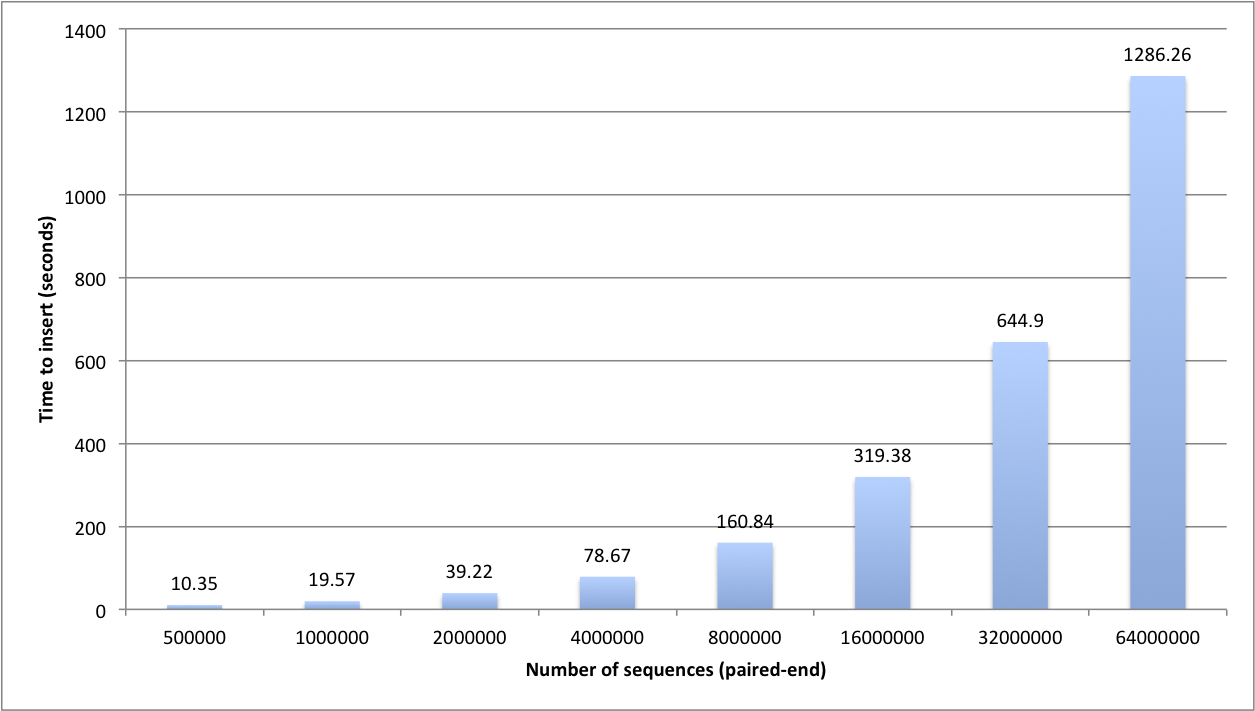
\includegraphics[width=\textwidth]{insertion_speed_chart}
	\caption{Chart of insertion speeds}
	\label{fig:insertion_speeds}
\end{figure}

\begin{table}[h]
\centering
\begin{tabular}{n{4}{2}n{4}{2}n{4}{2}}
	\toprule
 {Number of sequences (paired-end)} & {Input FASTQ size (MB)} & {Pip database (MB)} \\
 \midrule
 \np{500000} & 371.4 & 206.9 \\
 \np{1000000} & 743.00 & 413.9 \\
 \np{2000000} & 1486.00 & 828.00 \\
 \np{4000000} & 3051.52 & 1699.84 \\
 \np{8000000} & 6082.56 & 3389.44 \\
 \np{16000000} & 12165.12 & 6789.12 \\
 \np{32000000} & 24350.72 & 13568.0 \\
 \np{64000000} & 48701.44 & \\
 \np{91000000} & 69754.88 & 35061.76 \\
 \bottomrule
\end{tabular}
\caption{Comparison of input file sizes against Pip database sizes}
\label{tab:filesizes}
\end{table}

\begin{figure}[h]
	\centering
	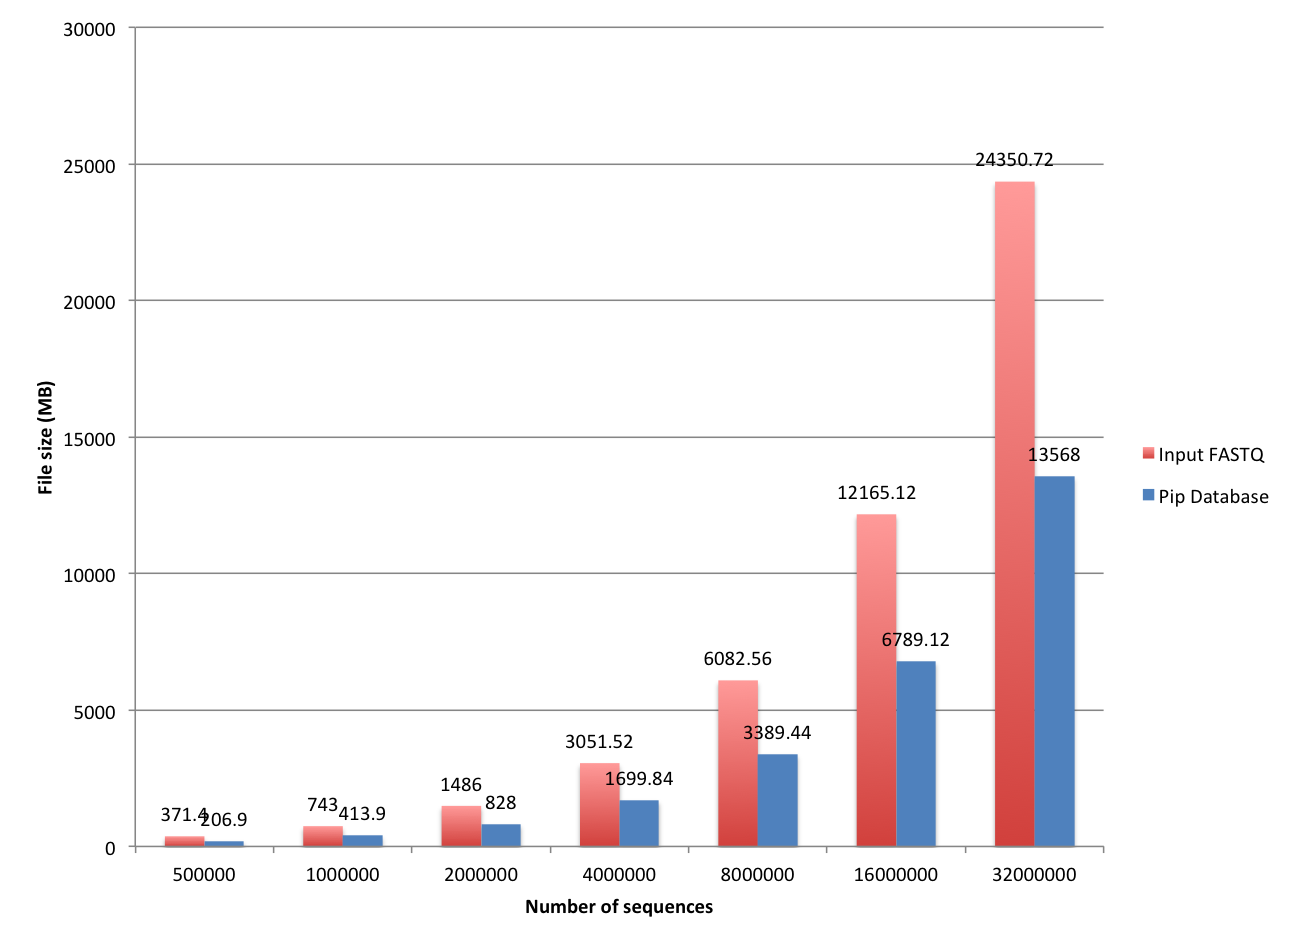
\includegraphics[width=\textwidth]{filesizes_chart}
	\caption{Chart of file sizes}
	\label{fig:filesizes}
\end{figure}


% section benchmarks (end)
\newpage
\section{Conclusion} % (fold)
\label{sec:conclusion}
The use of Pip within the 16S pipeline shows promise in reducing the logistical
effort of researcher and interoperability headaches of multiple tools.
% section conclusion (end)
\end{document}